\begin{sol}
\begin{enumerate}[label=\textbf{(\alph*)}] 
\item We begin by first drawing a diagram:
\begin{center}
    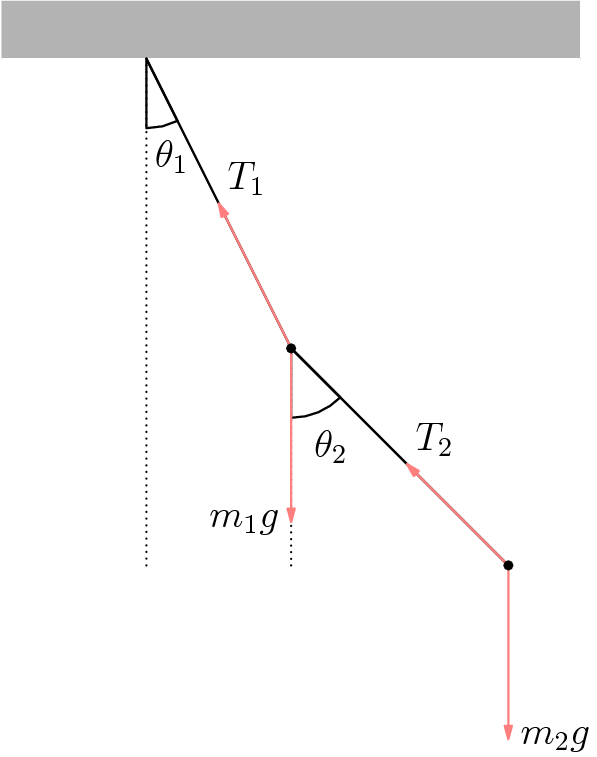
\includegraphics[width=8cm]{P03/double pendulum.png}
\end{center}
Since the angles are small, it holds that 
\[\sin\theta \approx \theta, \quad \cos\theta \approx 1.\]
Let us also define 
\[\sin\theta_1 = \frac{X_1}{L}, \quad \sin\theta_2 = \frac{X_2 - X_1}{L}.\]
The angles are small so $T_1 \approx (M_1 + M_2)g$ (as it holds both masses) and $T_2 \approx M_2 g$ (as it holds only the mass $M_2$). We can now write our equations of motion. We can start with the lower mass. The only force that attempts to bring the second mass back to
equilibrium is the horizontal component of $T_2$. Therefore, we have
\[M_2 \ddot{X}_2  = -T_2\sin\theta_2 = -\frac{M_2g}{\ell} (X_2 - X_1).\]
If we define $\omega^2 \equiv g/L$, we find 
\[\ddot{X}_2 + \omega_0^2 X_2 - \omega_0^2 X_1 = 0.\]
For the first mass, we have two forces. Although not labeled in the diagram there is a component $T_2$ that is directed along the rod and away from the first mass. Therefore, the two forces $T_1$ and $T_2$ fight for equilibrium and our equation of motion can be given as 
\begin{align*}
    M_1\ddot{X}_1 &= -T_1 \sin\theta_1 + T_2 \sin \theta_2 \\ 
     M_1 \ddot{X}_1 &= -2(M_1 + M_2)g \frac{X_1}{L} + M_2g\frac{X_2 - X_1}{L} \\
   0 &= \ddot{X}_1 + \frac{M_1 + 2M_2}{M_1}X_1\omega_0^2 - \frac{M_2}{M_1}X_2 \omega_0^2 
\end{align*}

   \item Using the definition of a normal mode 
\[
\begin{pmatrix}
X_1 \\
X_2 
\end{pmatrix}
= 
\Re \left[
\begin{pmatrix}
A_1 \\
A_2 
\end{pmatrix}
e^{i (\omega t + \phi)}
\right]
\]
we can rearrange to find that 
\begin{align*}
    0 &= \left(\frac{M_1 + 2M_2}{M_1}\omega_0^2 - \omega^2\right)A_1 - \frac{M_2}{M_1}\omega_0^2 A_2\\
    0 &= -\omega_0^2 A_1 + \left(\omega_0^2 - \omega^2\right)
\end{align*}
Now, rewrite in matrix format 
\[
\begin{pmatrix}
 \frac{M_1 + 2M_2}{M_1}\omega_0^2 - \omega^2 & -\frac{M_2}{M_1}\omega_0^2 \\ 
 -\omega_0^2 & \omega_0^2 - \omega^2
\end{pmatrix}
\begin{pmatrix}
A_1 \\
A_2
\end{pmatrix}
=0.
\]
To get a solution, we need to solve the equation where the determinant of the left matrix is zero.
\[
\begin{vmatrix}
\frac{M_1 + 2M_2}{M_1}\omega_0^2 - \omega^2 & -\frac{M_2}{M_1}\omega_0^2 \\ 
 -\omega_0^2 & \omega_0^2 - \omega^2
\end{vmatrix}
= 0.
\]
\[\left(\frac{M_1 + 2M_2}{M_1}\omega_0^2 - \omega^2\right)\left(\omega_0^2 - \omega^2\right) - \frac{M_2}{M_1}\omega_0^4 = 0\]
Rearranging yields the equation 
\[\omega^4 - \frac{2 (M_1 + M_2)}{M_1}\omega_0^2 \omega^2 + \frac{M_1 + M_2}{M_1}\omega_0^4 = 0.\]
Using substitution tells us that the roots of this equation are 
$$ \omega^2 = \frac{(M_2+M_1) \pm \sqrt {M_2^2 + M_1M_2}}{M1} \omega_0^2 \implies \omega^2 = (1+\alpha) \pm \sqrt {1+ \alpha^2}$$
Here we used $\alpha = \frac{M_2}{M_1}$
\end{enumerate}
\end{sol}